\documentclass{article}

\usepackage{amsfonts}
\usepackage[colorlinks=true,citecolor=blue,urlcolor=cyan,linkcolor=red]{hyperref}
\usepackage{amssymb}
\usepackage{amsmath,amssymb,amscd,epsfig,amsfonts,rotating}
\usepackage{graphicx}
\usepackage{epsfig}
\usepackage{multirow}
\usepackage{booktabs}
\usepackage{footnote}
\usepackage{subfigure}
\usepackage{float}
\usepackage{url}
\usepackage[margin=1.0in]{geometry}

\newtheorem{def:def}{Definition}
\newtheorem{thm:thm}{Theorem}
\newtheorem{thm:lm}{Lemma}

\DeclareMathOperator*{\argmax}{arg \, max}
\DeclareMathOperator*{\var}{var}
\DeclareMathOperator*{\cov}{cov}
\newcommand{\bs}{\boldsymbol}


\title{An Comparative Study on Audio Event Recognition}
\author{
{\small Jiacheng Yang} \\
{\small Shanghai Jiao Tong University}\\
{\small \textsf{kipsora@gmail.com}}}
\date{}
\begin{document}
	\maketitle

	\begin{abstract}
		As a human-level behaviour, audio event recognition is more and more popular and vital for artificial intelligence nowadays. Recently, Google has released AudioSet\cite{45857}, an equivalent of ImageNet\cite{5206848} in audio field. In this paper, we will have a comparative study on several basic network artitectures including DNN (including residual links\cite{DBLP:journals/corr/HeZRS15}), CNN\cite{Krizhevsky:2012:ICD:2999134.2999257} and RNN\cite{DBLP:journals/corr/SakSB14,DBLP:journals/corr/ChungGCB14} on AudioSet using three the most famous deep learning frameworks, Tensorflow\cite{45381}, MXNet\cite{DBLP:journals/corr/ChenLLLWWXXZZ15} and PyTorch. Additionally, we will also use ensemble methods to enhance our models.
	\end{abstract}

	\section{Introduction}\label{sec:intro}
		As deep learning methods are increasingly powerful, more and more problems can be solved by deep neural networks. Nevertheless, due to lacking of sufficient data, audios, as another dimension of real world inputs for humans, can still be a tremendous challenge for deep learning. For example, audio event recognition models always requires large amount of supervised training labels. 

		Recent works has shown that several methods in computer vision, for example, convolutional neural networks, can be successfully applied to audio classification problems\cite{45611}. However, besides computer vision whether basic methods/network architectures in other artificial intelligence subfields such like recurrent neural networks (or LSTM) frequently used in natural language processing will work on audio event recognition problem is still obscure.

		Recently, Google has released AudioSet\cite{45857}, which includes 2 million audio data with high-quality human labels. This dataset can be seen as the counterpart of ImageNet in audio event recognition field. In this paper, we will have several comparative experiments on AudioSet for basic network architectures and machine learning methods.

	\section{Methodology}\label{sec:method}
		\subsection{Formulation}\label{sec:formulate}
			Audio event recognition can be seen as a multi-label classification problem where each label stands for a tag like ``Boom'' and ``Swing Music''. Each data entry has an input feature extracted from the bottom layer of ResNet\cite{45857,DBLP:journals/corr/HeZRS15} and a human-labeled ground truth. Formally speaking, during training we want to train a classifier $f_\theta$ under supervised dataset $\mathcal{D}=\{(\mathbf{x}^{(i)}, \mathbf{y}^{(i)})\}$ by minimize a objective loss function $\mathcal{L}(f_\theta(\mathbf{x}), \mathbf{y})$, where $\theta$ is the parameters of the classifier; $\mathbf{x}$ stands for the input feature vector and $\mathbf{y}$ is the target list consists of several tags. In testing/predicting phase, given an input $\mathbf{x}$, this classifier will produce an tag lists (or probabilities for every tags) $\hat{\mathbf{y}} = f_\theta(\mathbf{x})$.

		\subsection{Objective Loss Function}
			We used Sigmoid Binary Cross Entropy(SBCE for abbreviation) as our objective loss function, which regards a multi-label classification problem as a set of binary classification problems. Other methods described in \cite{online:multilabel} are remained as future works. 

			Given a classifier $f_\theta)$, SBCE on data batch $(\mathbf{x}_i, \mathbf{y}_i)$ is defined as:
			\[\mathcal{L}_\mathrm{SBCE}(\hat{\mathbf{y}}, \mathbf{y}) = -\dfrac{1}{n}\sum_{i = 1}^n\sum_{j = 1}^{C} \mathbf{y}_{ij} \log{\hat{\mathbf{y}}_{ij}} + (1 - \mathbf{y}_{ij})\log{(1 - \hat{\mathbf{y}}_{ij})}\]
			where $\mathbf{y}_{ij}$ means the value of the $j$-th class of one-hot vector; $\mathbf{\hat{y}}_{ij}$ means the counterpart for predict vector; $n$ is the batch size and $C$ is the number of classes.

		\subsection{Network Architectures}
			We compared three network architectures, DNN, CNN and RNN on AudioSet using three mainstream deep learing frameworks, Tensorflow, MXNet and PyTorch.

			\subsubsection*{Deep Neural Networks}
				We will use single layer to 8-layers neural networks with ReLU as their activation function. Batchnorm layer\cite{DBLP:journals/corr/IoffeS15} and Dropout layer\cite{DBLP:journals/corr/abs-1207-0580} as well as Residual Links\footnote{We may add residual connections skipping more than one layers to improve the performance.} are also seen as variables. The network architecture is illustrated in figure \ref{fig:dnn-arch} where the dashed lines means it is an experimental variable and star symbol means that the architecture inside the bracket will repeats for 0 or more times.

				\begin{figure}[htbp]
					\centering
					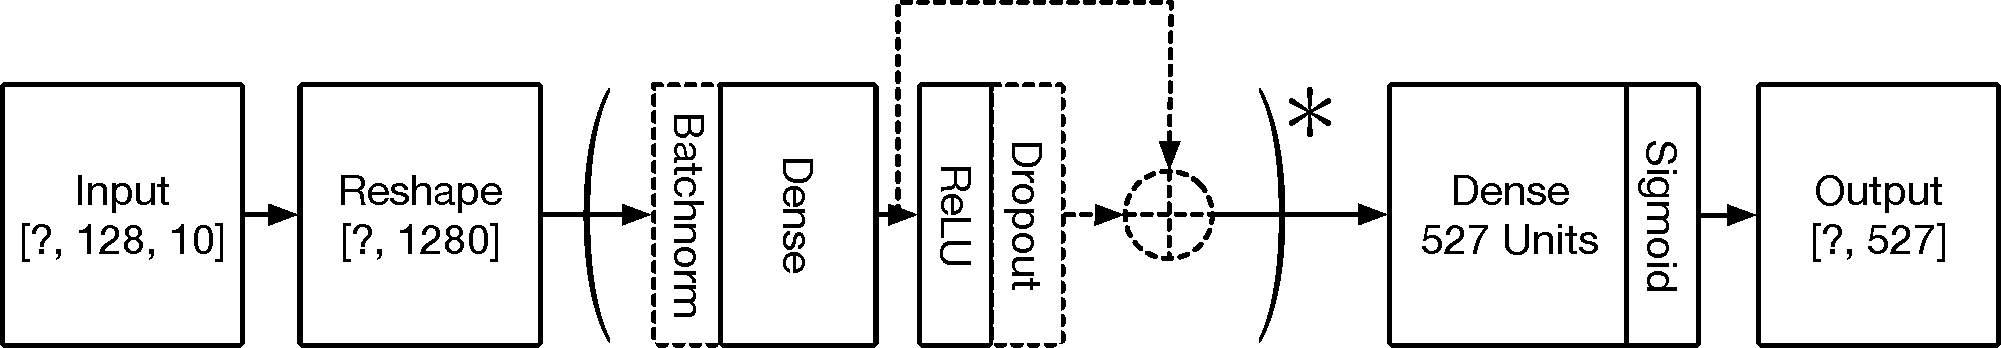
\includegraphics[width=13cm]{figures/dnn-arch.pdf}
					\caption{\label{fig:dnn-arch}The Architecture of Deep Neural Networks}
				\end{figure}

			\subsubsection*{Convolutional Neural Networks}
				According to \cite{45611}, CNN can be also performs well on audio classification. However, in our settings, considering the input feature is extracted from the bottom layer of ResNet, it is hard to say whether CNN will outperform DNN under this circumstance without experiments. We tried the network structure illustrated in the figure \ref{fig:cnn-arch}.
				\begin{figure}[htbp]
					\centering
					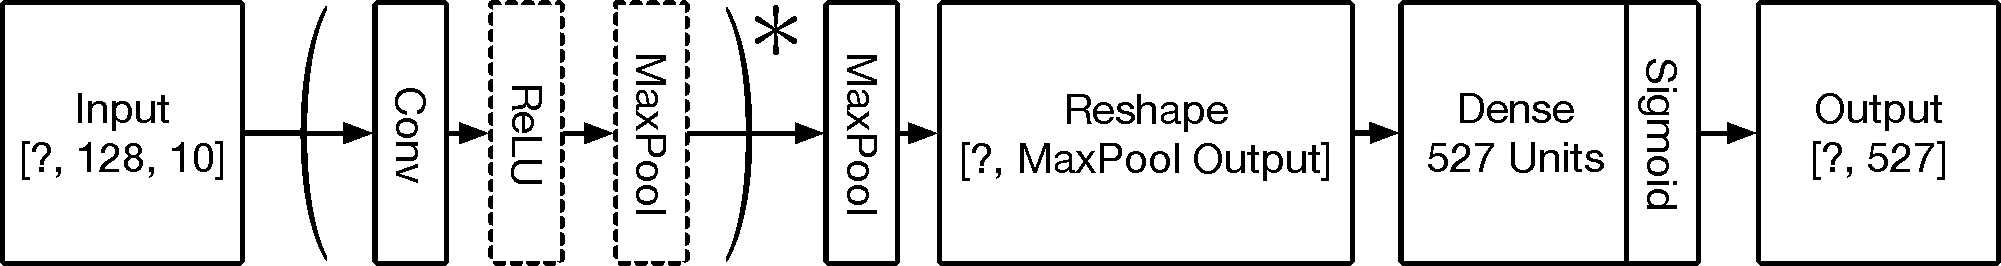
\includegraphics[width=13cm]{figures/cnn-arch.pdf}
					\caption{\label{fig:cnn-arch}The Architecture of Convolutional Neural Networks}
				\end{figure}

			\subsubsection*{Recurrent Neural Networks}
				As another powerful tool dealing with temporal data like text, RNN is also selected for a model to be compared with. We used LSTM as well as GRU as our RNN cell. The figure \ref{fig:rnn-arch} illustrates the basic RNN structure we used.
				\begin{figure}[htbp]
					\centering
					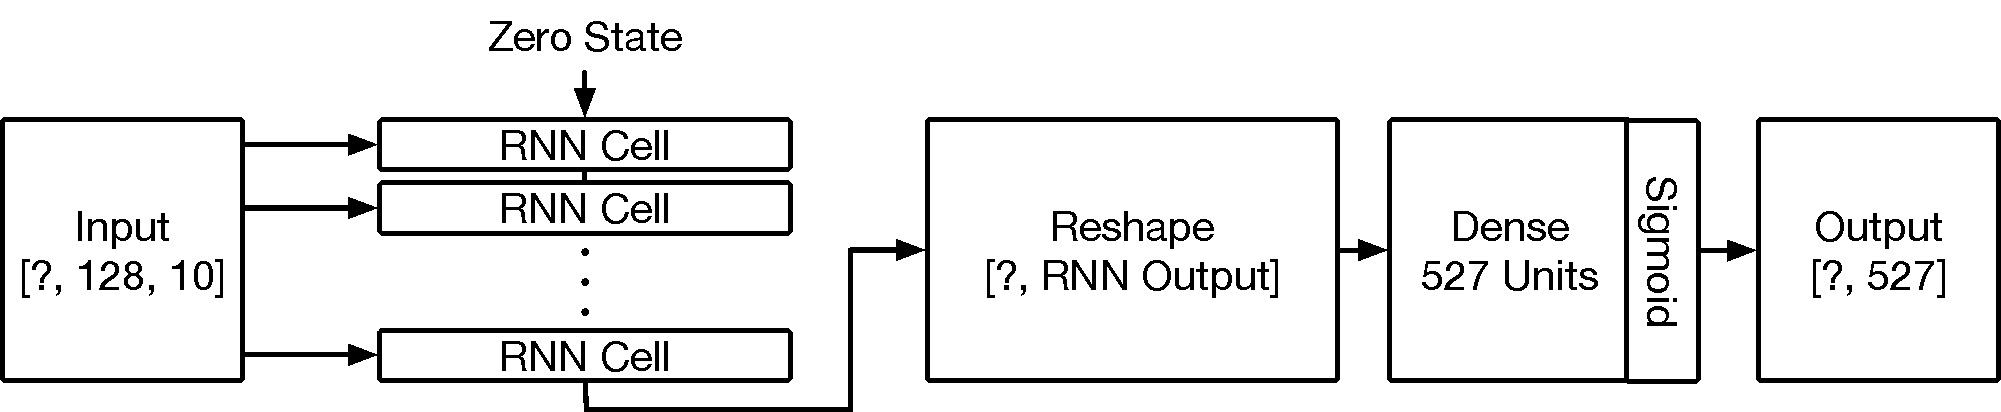
\includegraphics[width=13cm]{figures/rnn-arch.pdf}
					\caption{\label{fig:rnn-arch}The Architecture of Recurrent Neural Networks}
				\end{figure}

		\subsection{Metrics}
			We use two metrics to measure models' power:
			\begin{enumerate}
				\item \textbf{AP(Average Precision):} It computes the area under precision-recall curve. In the evaluation section, record the set segments classified for each category as $A_i$ and denote the set of segments in each category as $B_i$. Precision $p_i$ is defined as $p_i = \dfrac{|A_i \cap B_i|}{|A_i|}$ and recall is defined as $r_i = \dfrac{|A_i \cap B_i|}{|B_i|}$. Compute the area of precision-recall curve for recall from $0$ to $1$ gets the average precision for each category.
				\item \textbf{AUC(Area Under ROC Curve):} computes the area under the ROC curve, which is a TPR-FPR curve. Denote the set of all segments as $C$. TPR(true positive rate) is defined as $\dfrac{|A_i \cap B_i|}{|B_i|}$ and FPR is defined as $\dfrac{|A_i \cap B_i|}{|C - B_i|}$. Compute the area of ROC for FPR from $0$ to $1$ gets the AUC score for each category.
			\end{enumerate}

	\section{Experiments and Results}\label{sec:exps}
		\subsection{Deep Neural Networks}
			\subsubsection*{Training Settings}\label{sub:deep_neural_networks}
				We used RMSProp as our optimizer and the learning rate is $5\times 10^{-5}$ and L2 loss as regularizer, the strength of which is $1 \times 10^{-2}$ for every experiments. Initializer is truncated normal initializer, the stddev of which is about $1 \times 10^{-3}$($1 \times 10^{-2}$ for deep networks with residual connections). In addition, we separate $30\%$ of the training data as validation set to select the best hyperparameters (e.g. training epochs, dropout rate, batch size and hidden units in each layer). The final model will be trained with all of the training data.
			\subsubsection*{Results}
				The results on evalutaion set of different networks are listed in the table \ref{table:dnn-res} and the performance curves are shown in figure \ref{fig:dnn-proc}. As we can see in the table, the single layer NN performs the best. And the deep neural networks with residual links are not much worse than single layer neural networks. Besides, the baseline classifier logisitic regression also performs not bad on this dataset. These results prove that the dataset is relatively simple and a very deep network is liable to be overfitting here.
				\begin{table}[htbp]
					\centering
					\begin{tabular}{c|ccccc}
						\hline
						\hline
						          Layers   & None & BN & Dropout & BN-Dropout & Residual \\
						\hline
						$0$  & 90.5/0.174 & 90.4/0.169 & N/A & N/A & N/A \\
						$1$  & 94.4/0.236 & 94.5/0.241 & 94.5/0.242 & 94.4/0.240 & 93.5/0.207\\
						$2$  & 93.7/0.213 & 93.8/0.216 & 93.5/0.203 & 93.7/0.212 & 93.8/0.209\\
						$4$  & 93.4/0.193 & 93.5/0.195 & 92.9/0.173 & 93.2/0.185 & 93.5/0.226\\
						$7$\footnotemark  & N/A & N/A & N/A & N/A & 93.7/0.216 \\
						\hline
					\end{tabular}
					\caption{\label{table:dnn-res}Experiments on Deep Neural Networks}
				\end{table}
				\begin{figure}[htbp]
					\centering
					\subfigure[AUC]{
						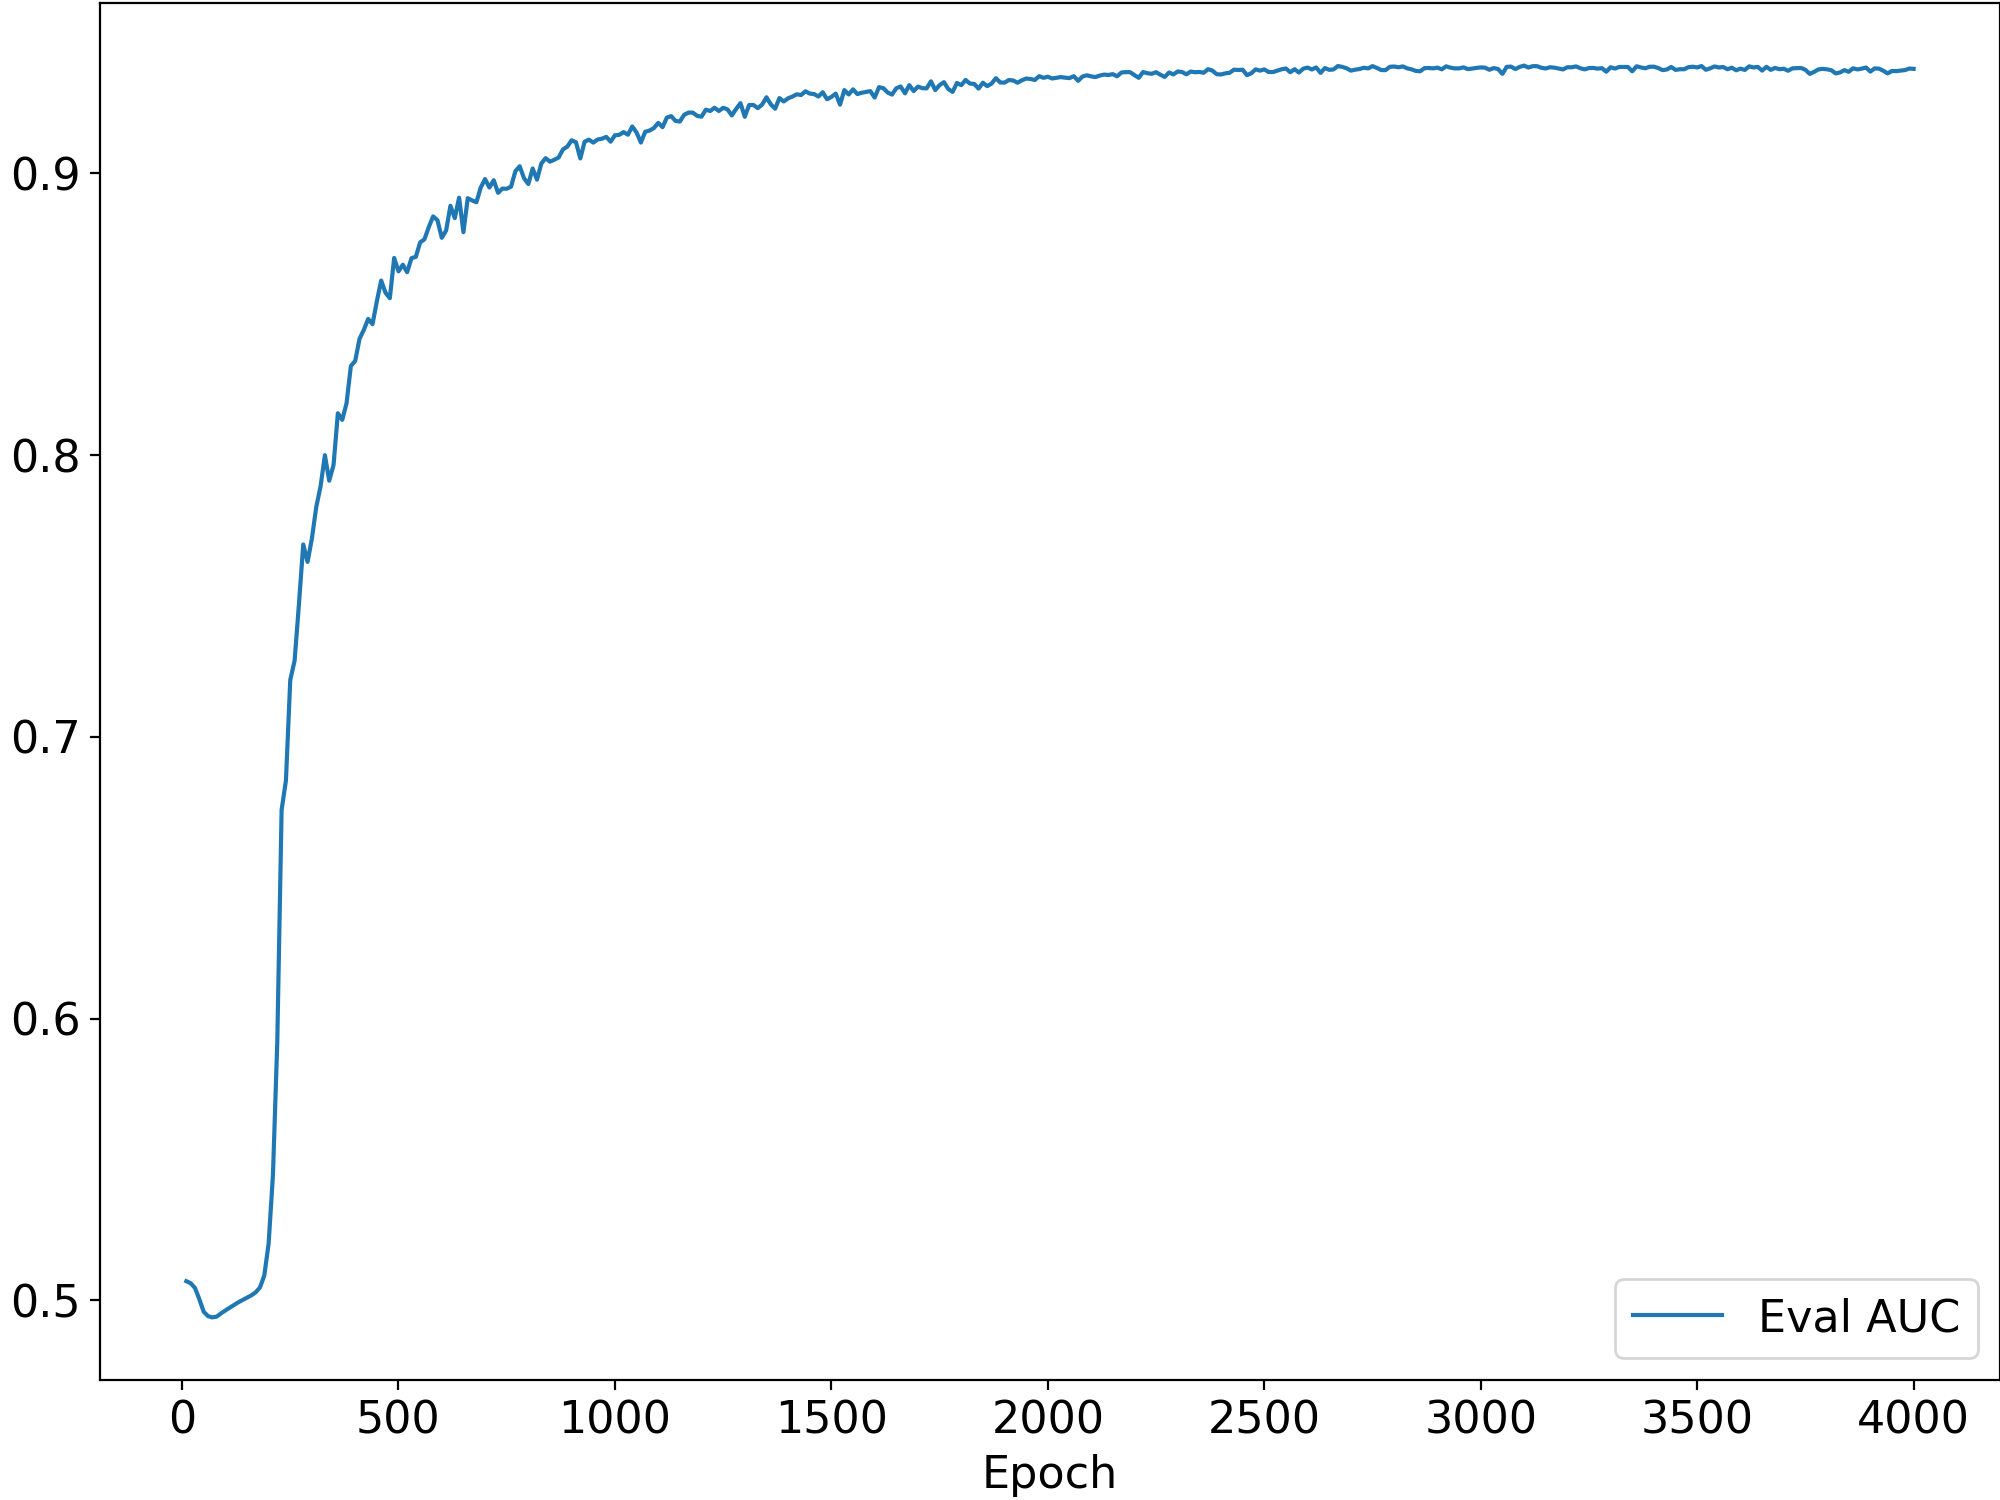
\includegraphics[width=4.8cm]{figures/dnn-AUC.png}
					}
					\subfigure[AP]{
						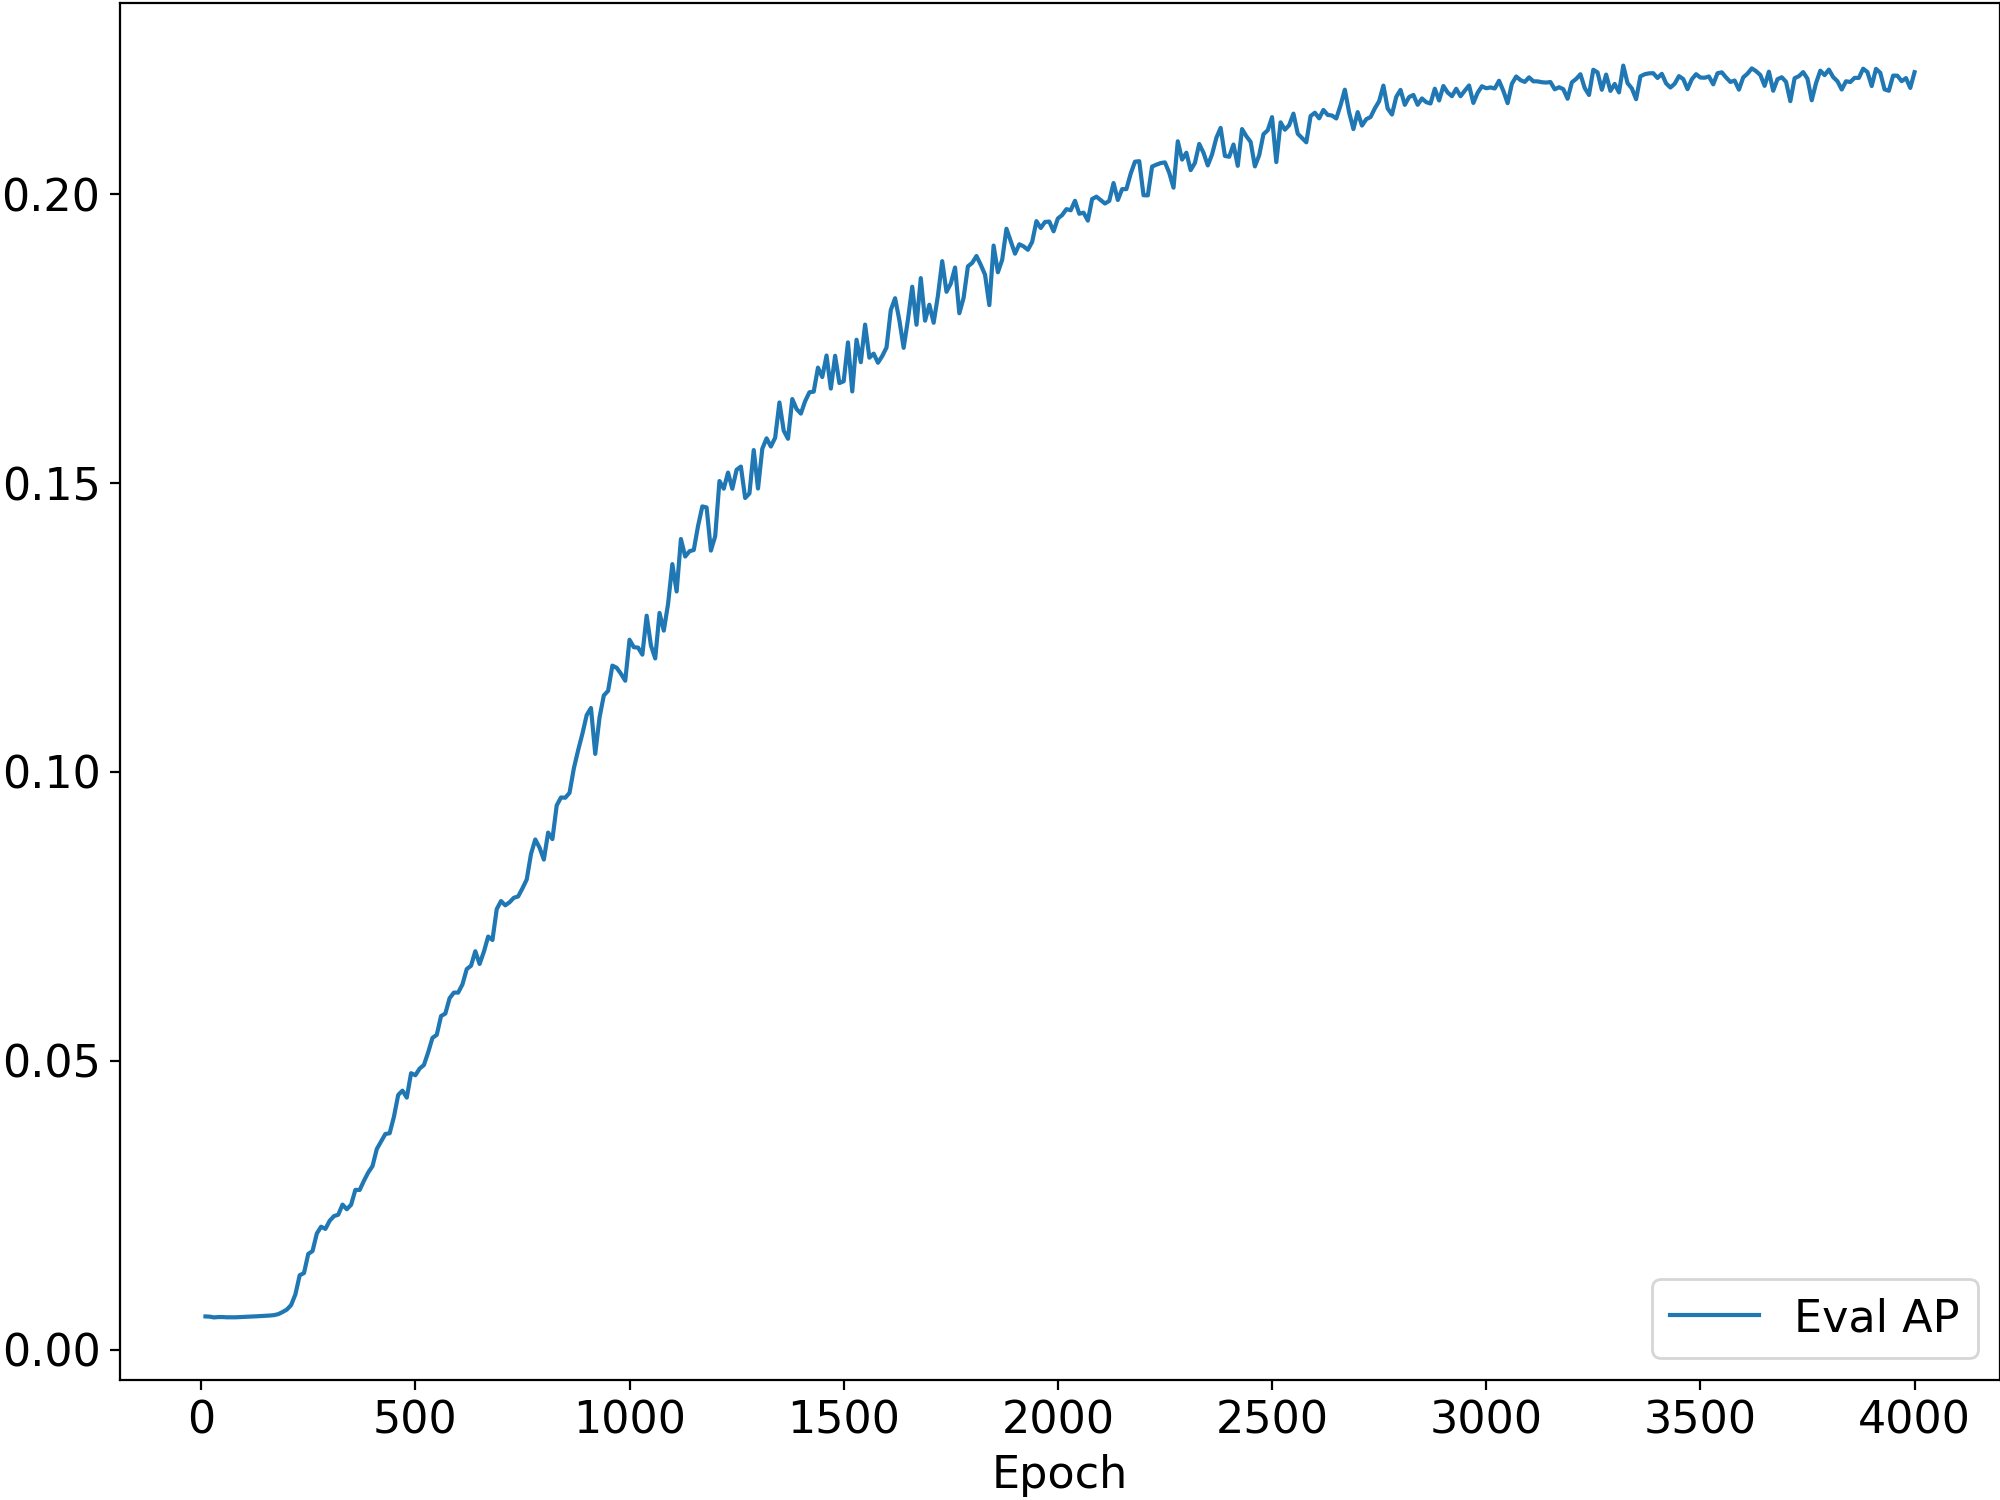
\includegraphics[width=4.8cm]{figures/dnn-AP.png}
					}
					\subfigure[Loss]{
						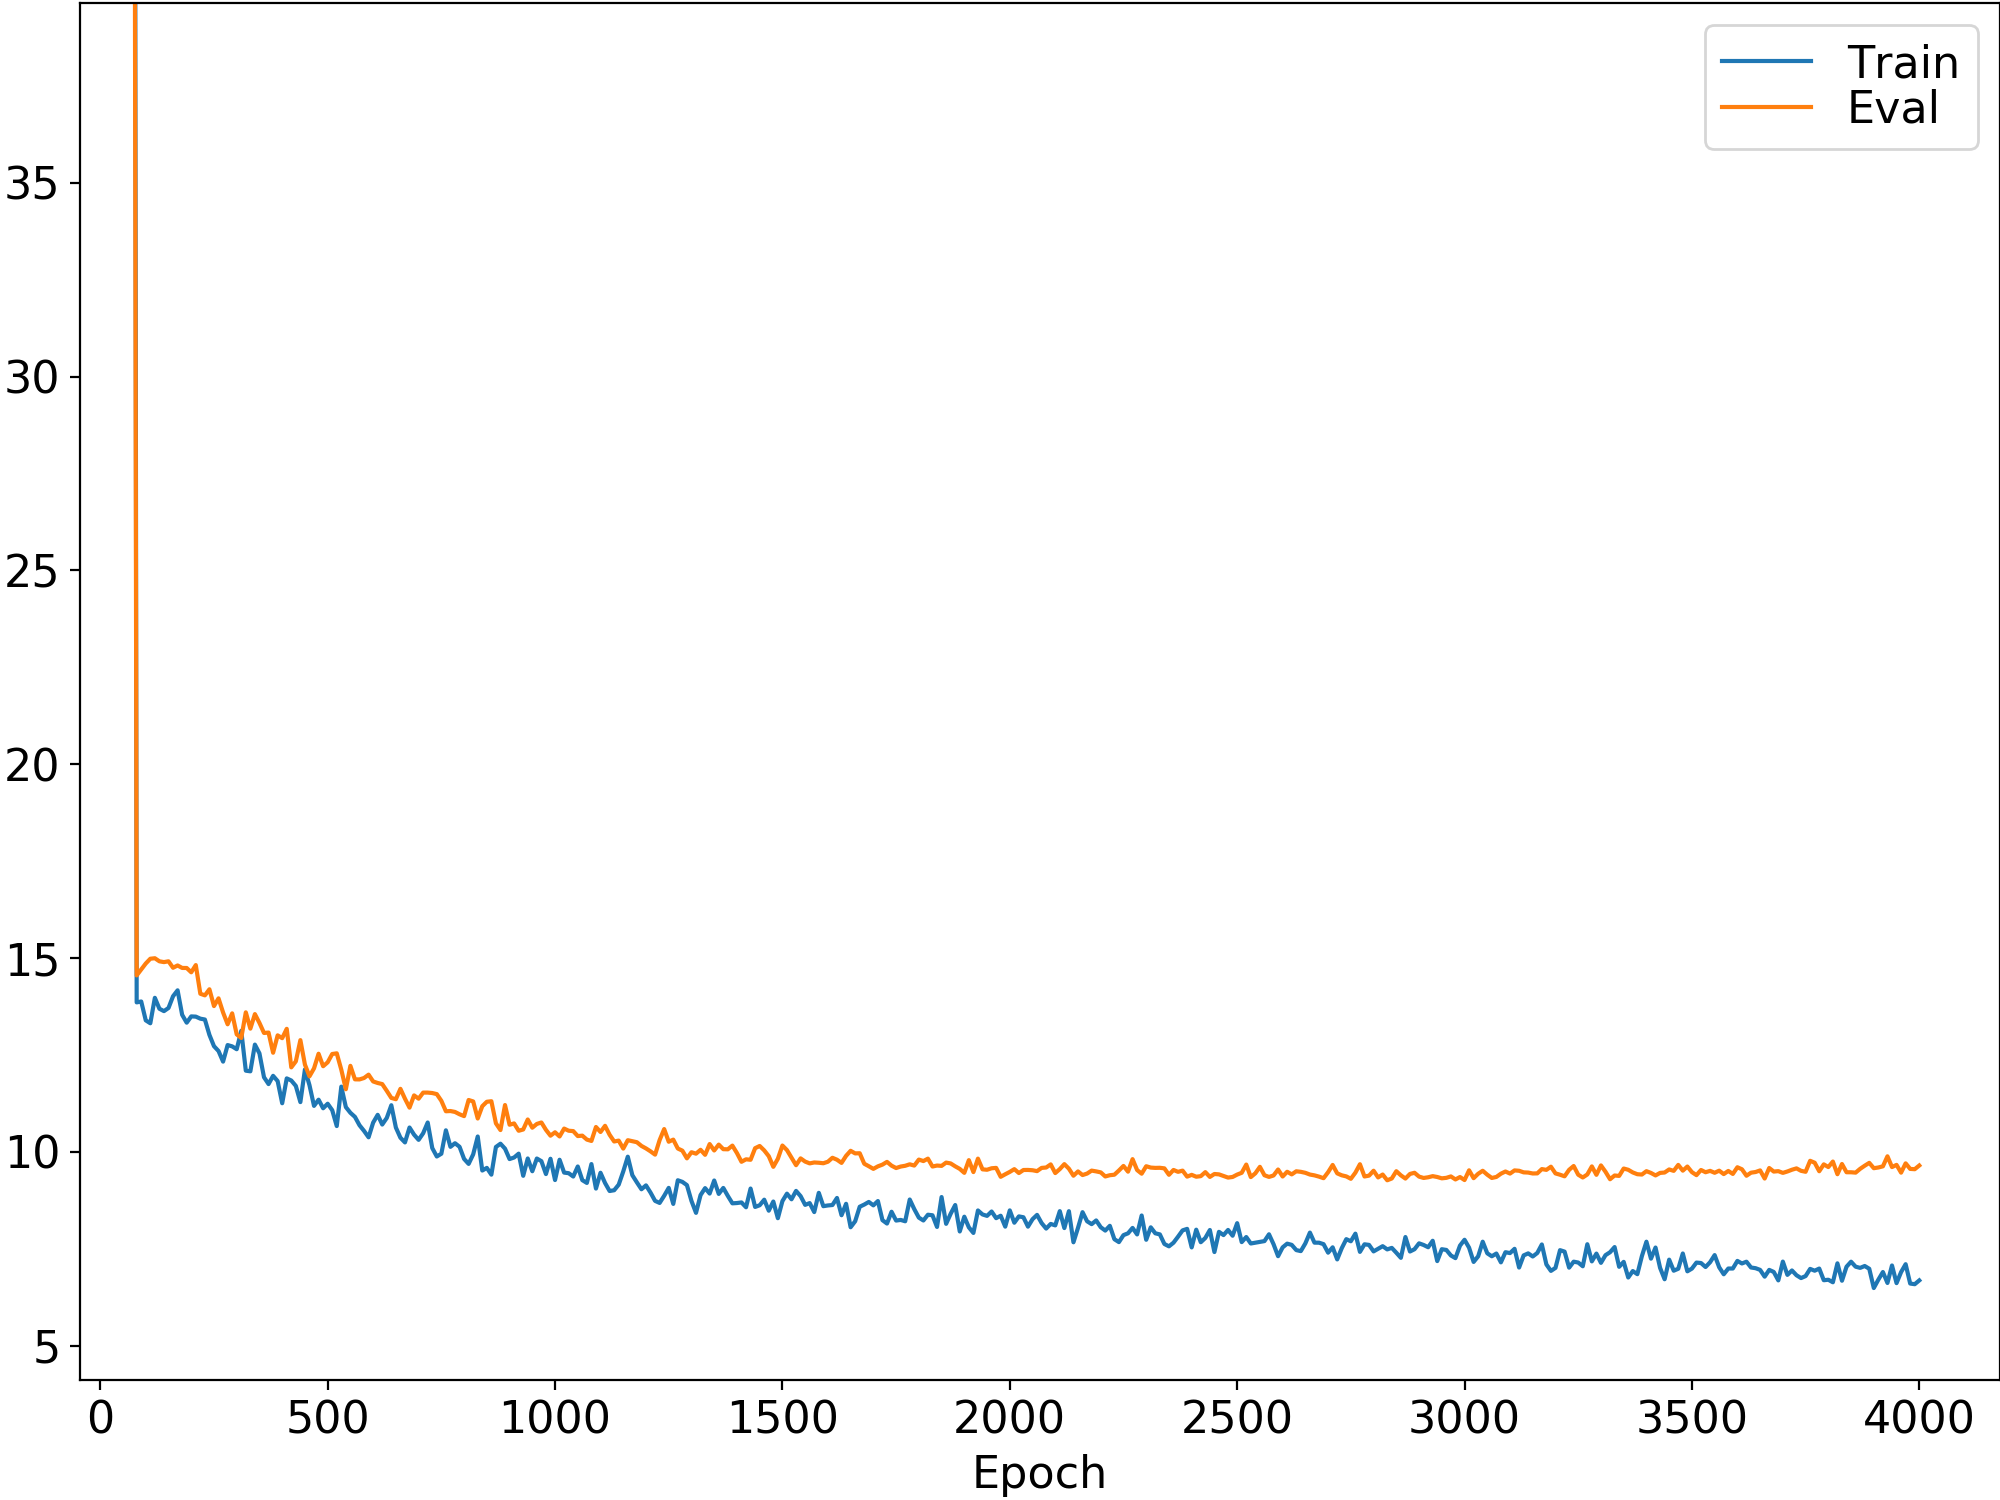
\includegraphics[width=4.8cm]{figures/dnn-loss.png}
					}
					\caption{\label{fig:dnn-proc}Figures on Deep Neural Networks}
				\end{figure}
				\footnotetext{Deep network will suffer from gradients vanishing problem if residual links are not added.}
		\subsection{Convolutional Neural Networks}
			\subsubsection*{Training Settings}
				We used three type of filters, the number of each of which is $128$ and the kernel size are swept over $[2, 3, 5]$ with stride $1$ followed by a maxpooling layer (if used) whose pool size is $[5, 3, 2]$ respectively.  Other training settings is the same as DNN.
			\subsubsection*{Results}
				The performance of CNN is listed in the table \ref{table:cnn-res} and the curves are shown in figure \ref{fig:cnn-proc}. Most of AUCs are slightly below the baseline line methods single layer DNN. But the APs are almost the same.
				\begin{table}[htbp]
					\centering
					\begin{tabular}{c|cccc}
						\hline
						\hline
						                  & None & (Conv-ReLU)$^\mathrm{*}$-Maxpool & (Conv-Maxpool-ReLU)$^\mathrm{*}$\\
						\hline
						Single Layer DNN & 94.5/0.242 & N/A & N/A \\
						2 Conv Layers    & N/A & 94.2/0.242 & 94.2/0.244 \\
						3 Conv Layers    & N/A & 94.2/0.235 & 94.1/0.231\\
						\hline
					\end{tabular}
					\caption{\label{table:cnn-res}Experiments on Convolutional Neural Networks}
				\end{table}
				\begin{figure}[H]
					\centering
					\subfigure[AUC]{
						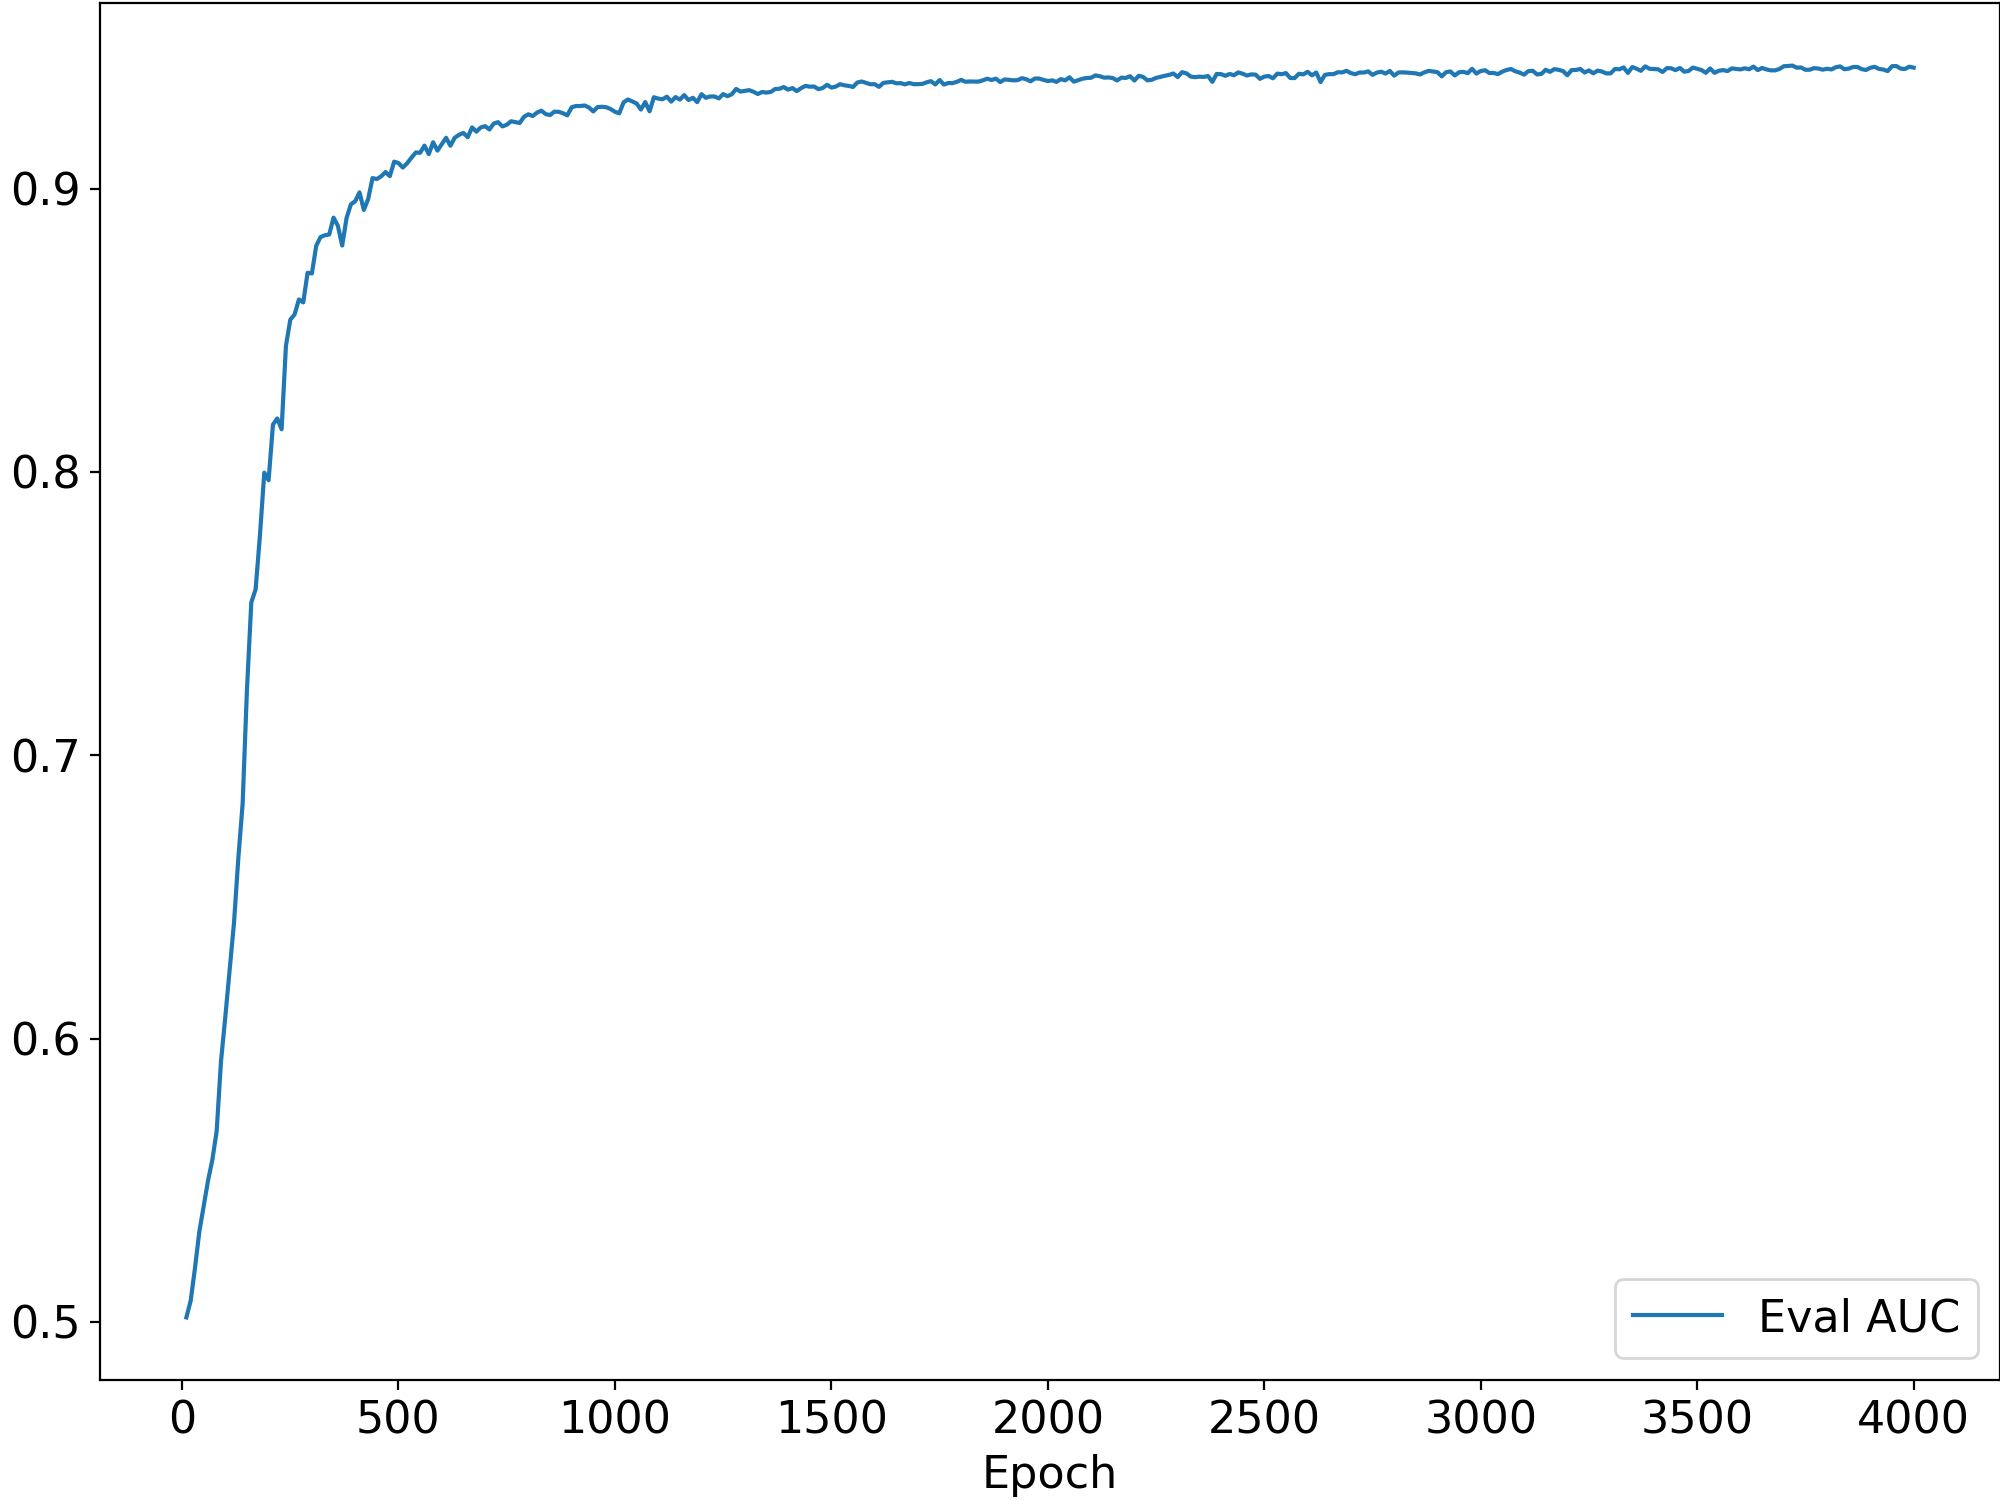
\includegraphics[width=4.8cm]{figures/cnn-AUC.png}
					}
					\subfigure[AP]{
						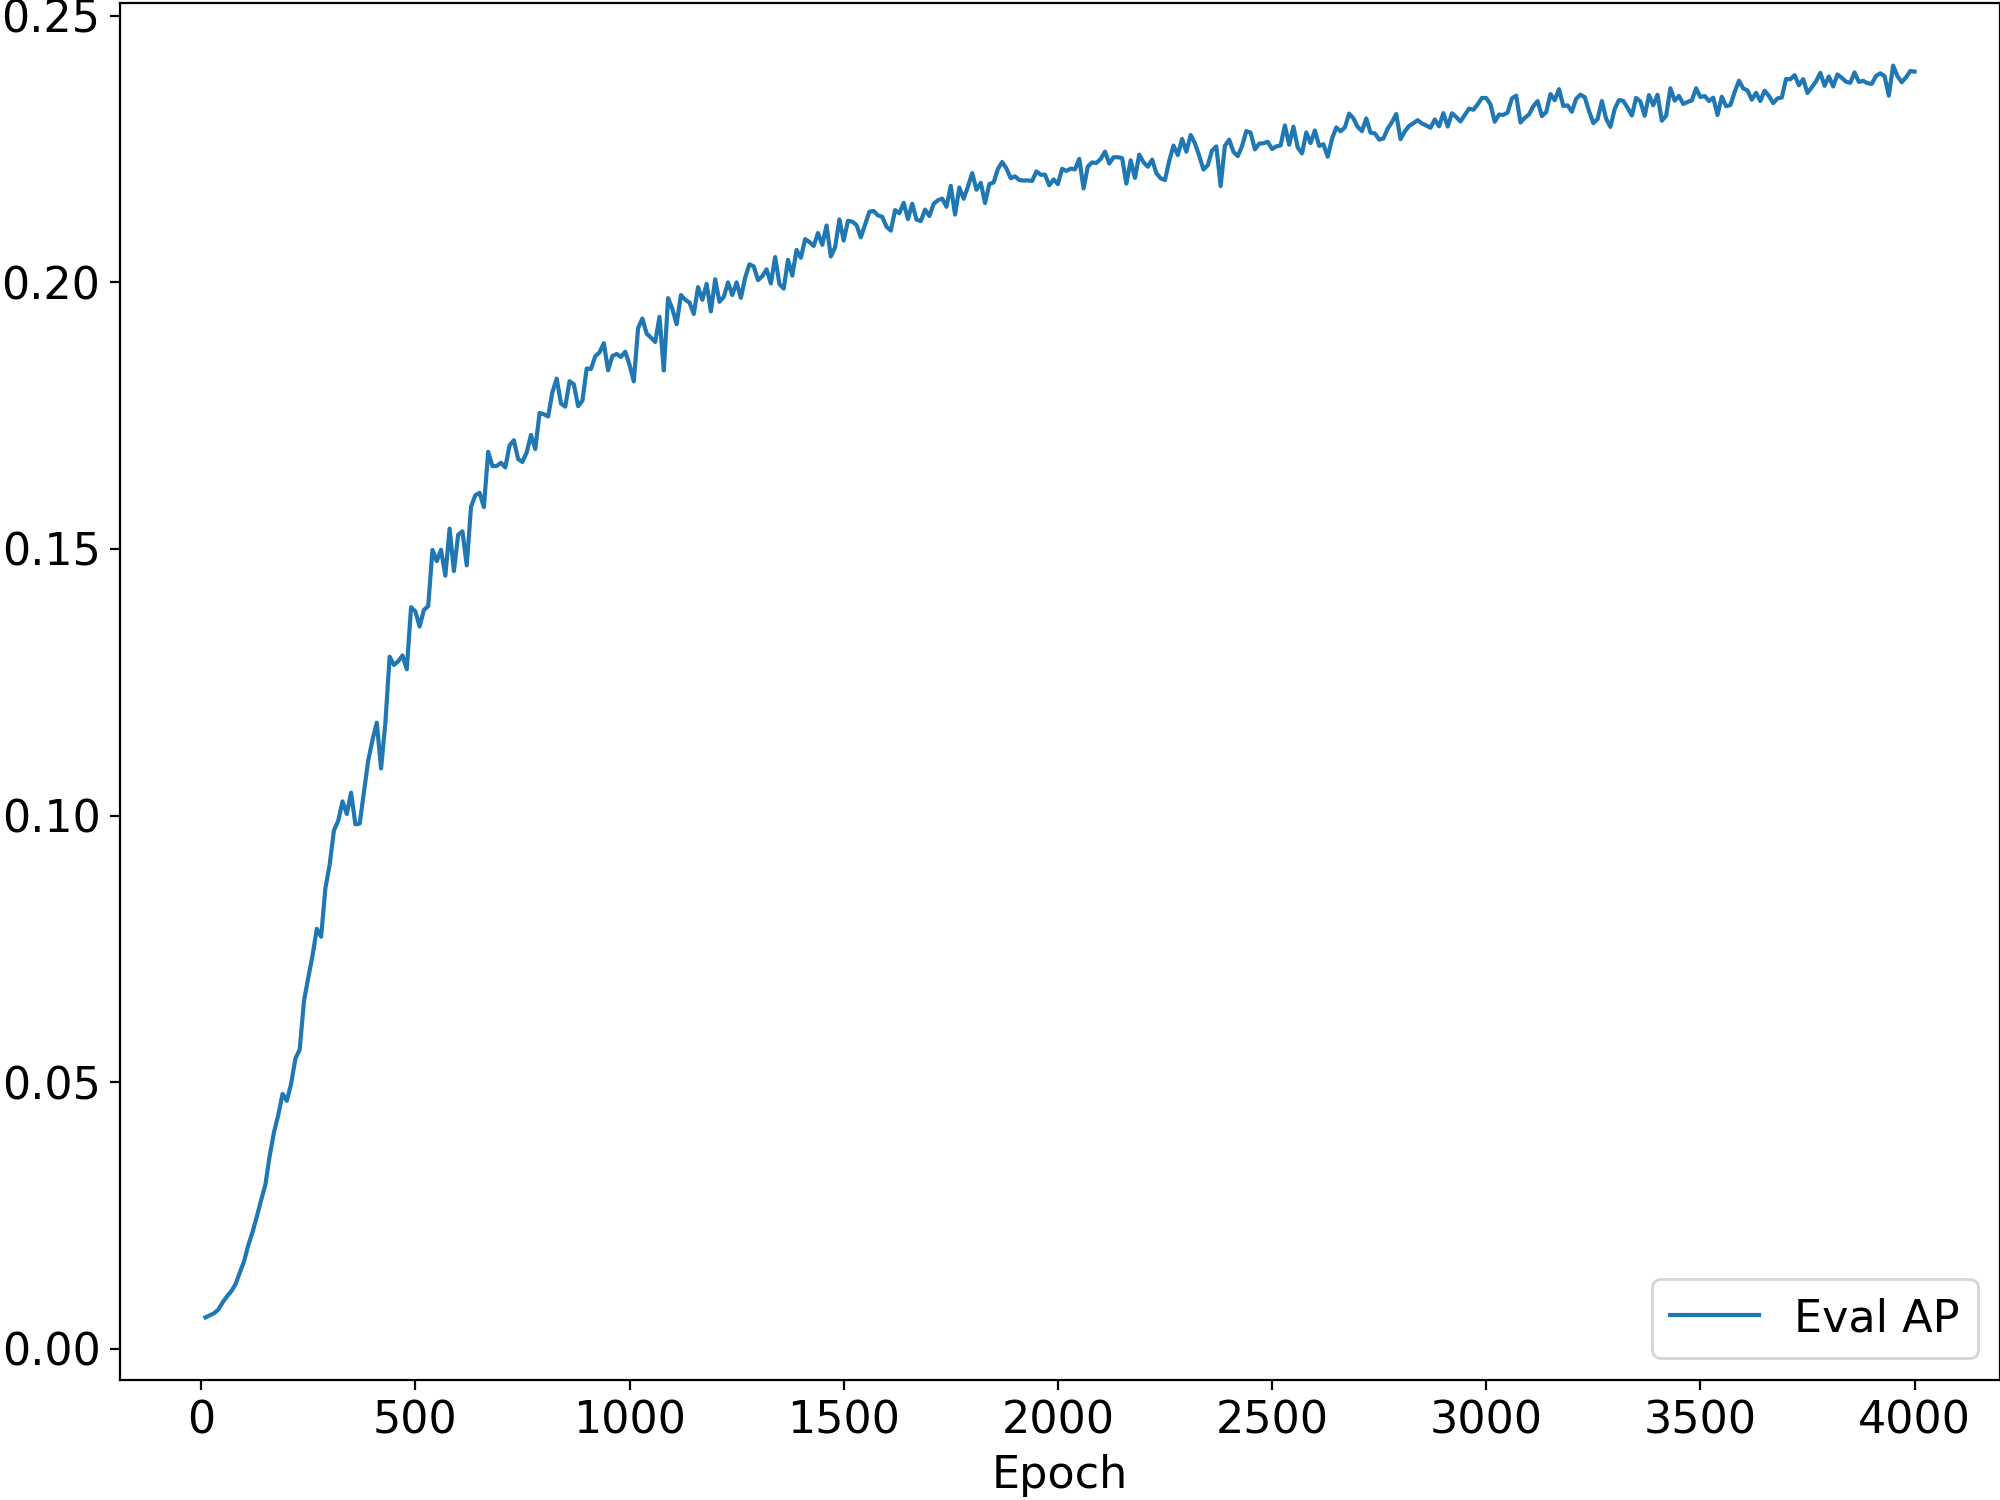
\includegraphics[width=4.8cm]{figures/cnn-AP.png}
					}
					\subfigure[Loss]{
						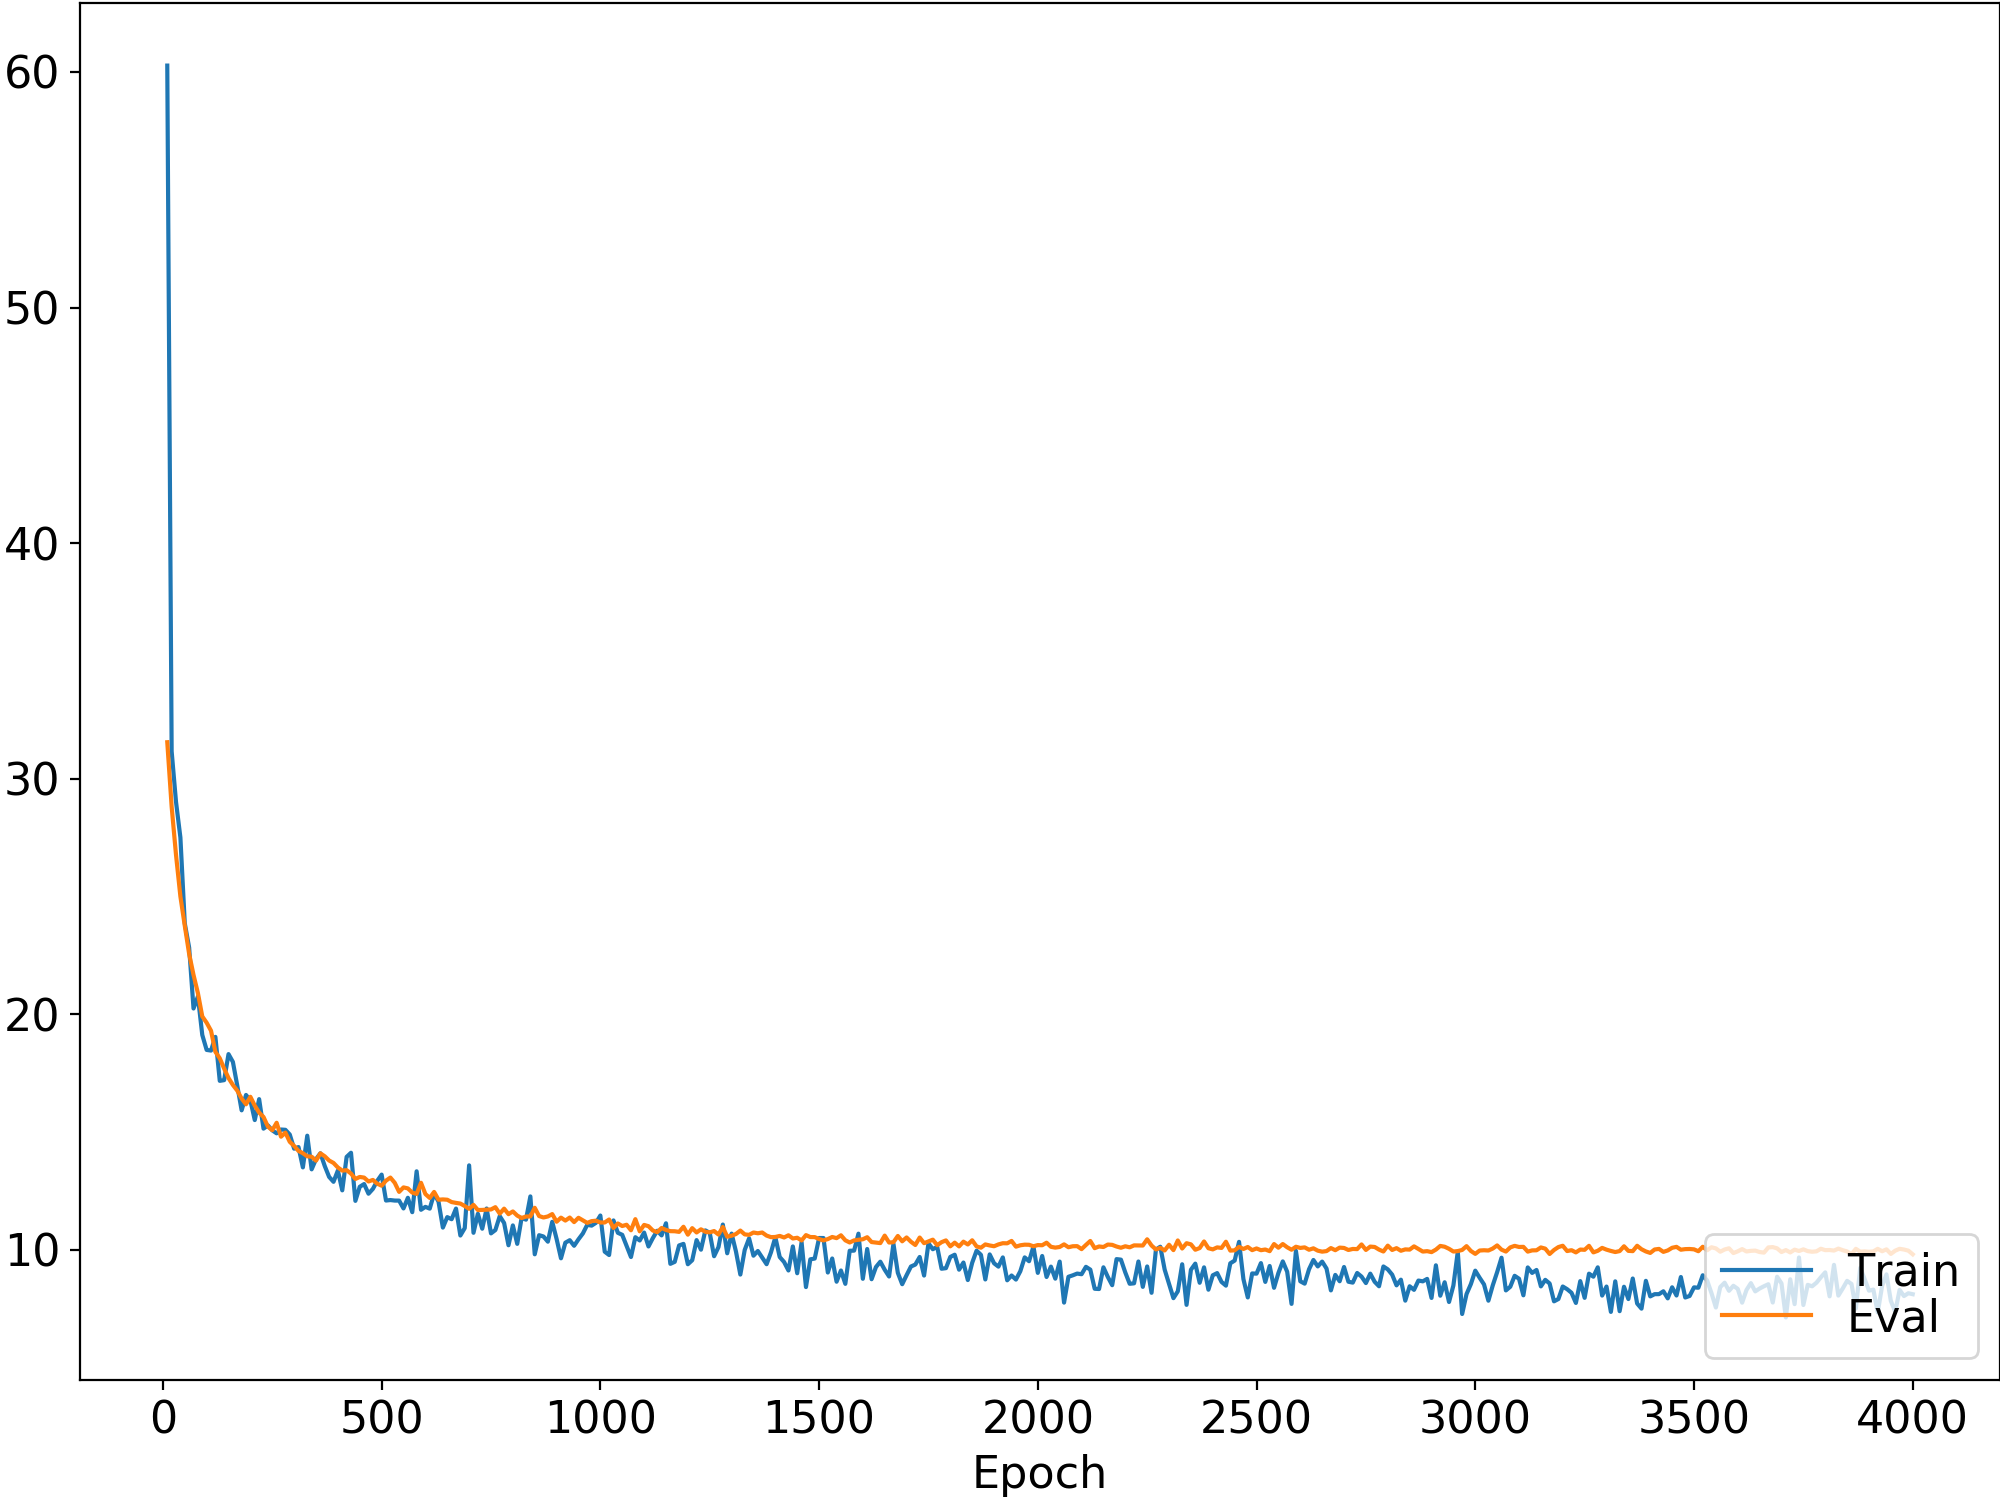
\includegraphics[width=4.8cm]{figures/cnn-loss.png}
					}
					\caption{\label{fig:cnn-proc}Figures on Convolutional Networks}
				\end{figure}

		\subsection{Recurrent Neural Networks}
			\subsubsection*{Training Settings}
				We also tried another basic neural network architecture, recurrent neural networks, on AudioSet. Multi-layers LSTM \cite{DBLP:journals/corr/SakSB14} is used as RNN cell in this experiment. The hyperparameters' settings are the same as the experiment \ref{sub:deep_neural_networks}.

			\subsubsection*{Results}
				The results on recurrent neural networks are shown in table \ref{table:rnn-res} and the training curve is shown in figure \ref{fig:rnn-proc}. As we can see in the table, the good performances are stable with varying hyperparameters. Actually we do not fine tune the parameters for RNN. Hence it means that RNN is potential a better method than simple layer DNN.
				\begin{table}[htbp]. 
					\centering
					\begin{tabular}{c|cccc}
						\hline
						\hline
						                  & None & 1024 Hidden Units & 2048 Hidden Units\\
						\hline
						Single Layer DNN & 94.5/0.242 & N/A & N/A \\
						6 Layers       & N/A & 94.2/0.234 & 94.4/0.246 \\
						10 Layers      & N/A & 94.1/0.233 & 94.4/0.244 \\
						\hline
					\end{tabular}
					\caption{\label{table:rnn-res}Experiments on Recurrent Networks}
				\end{table}
				\begin{figure}[htbp]
					\centering
					\subfigure[AUC]{
						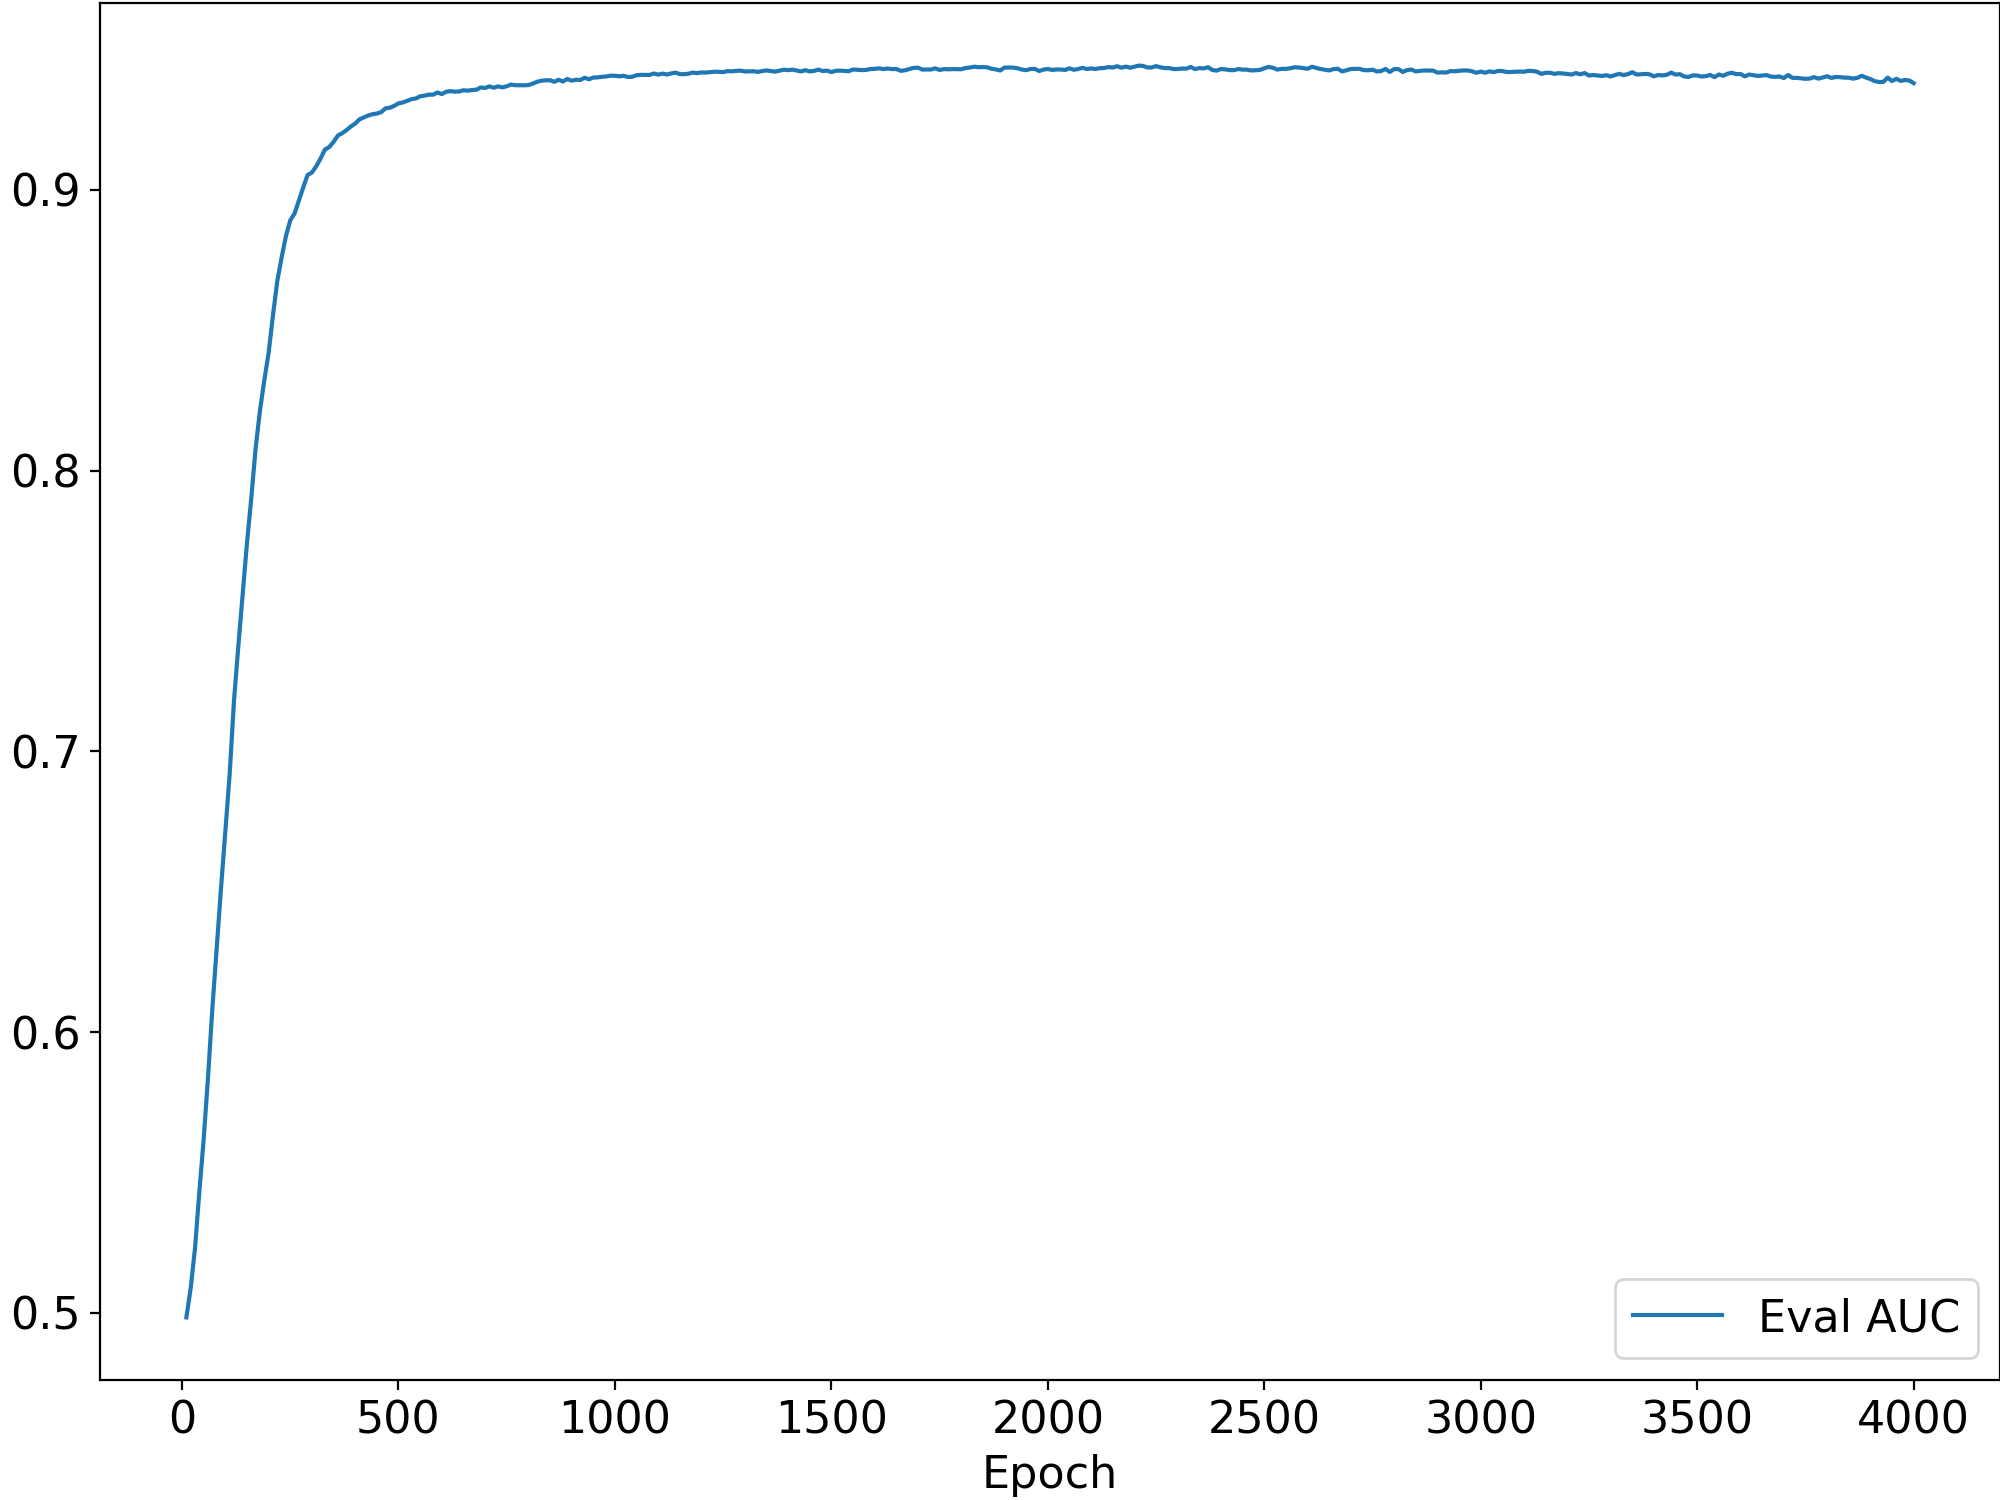
\includegraphics[width=4.8cm]{figures/rnn-AUC.png}
					}
					\subfigure[AP]{
						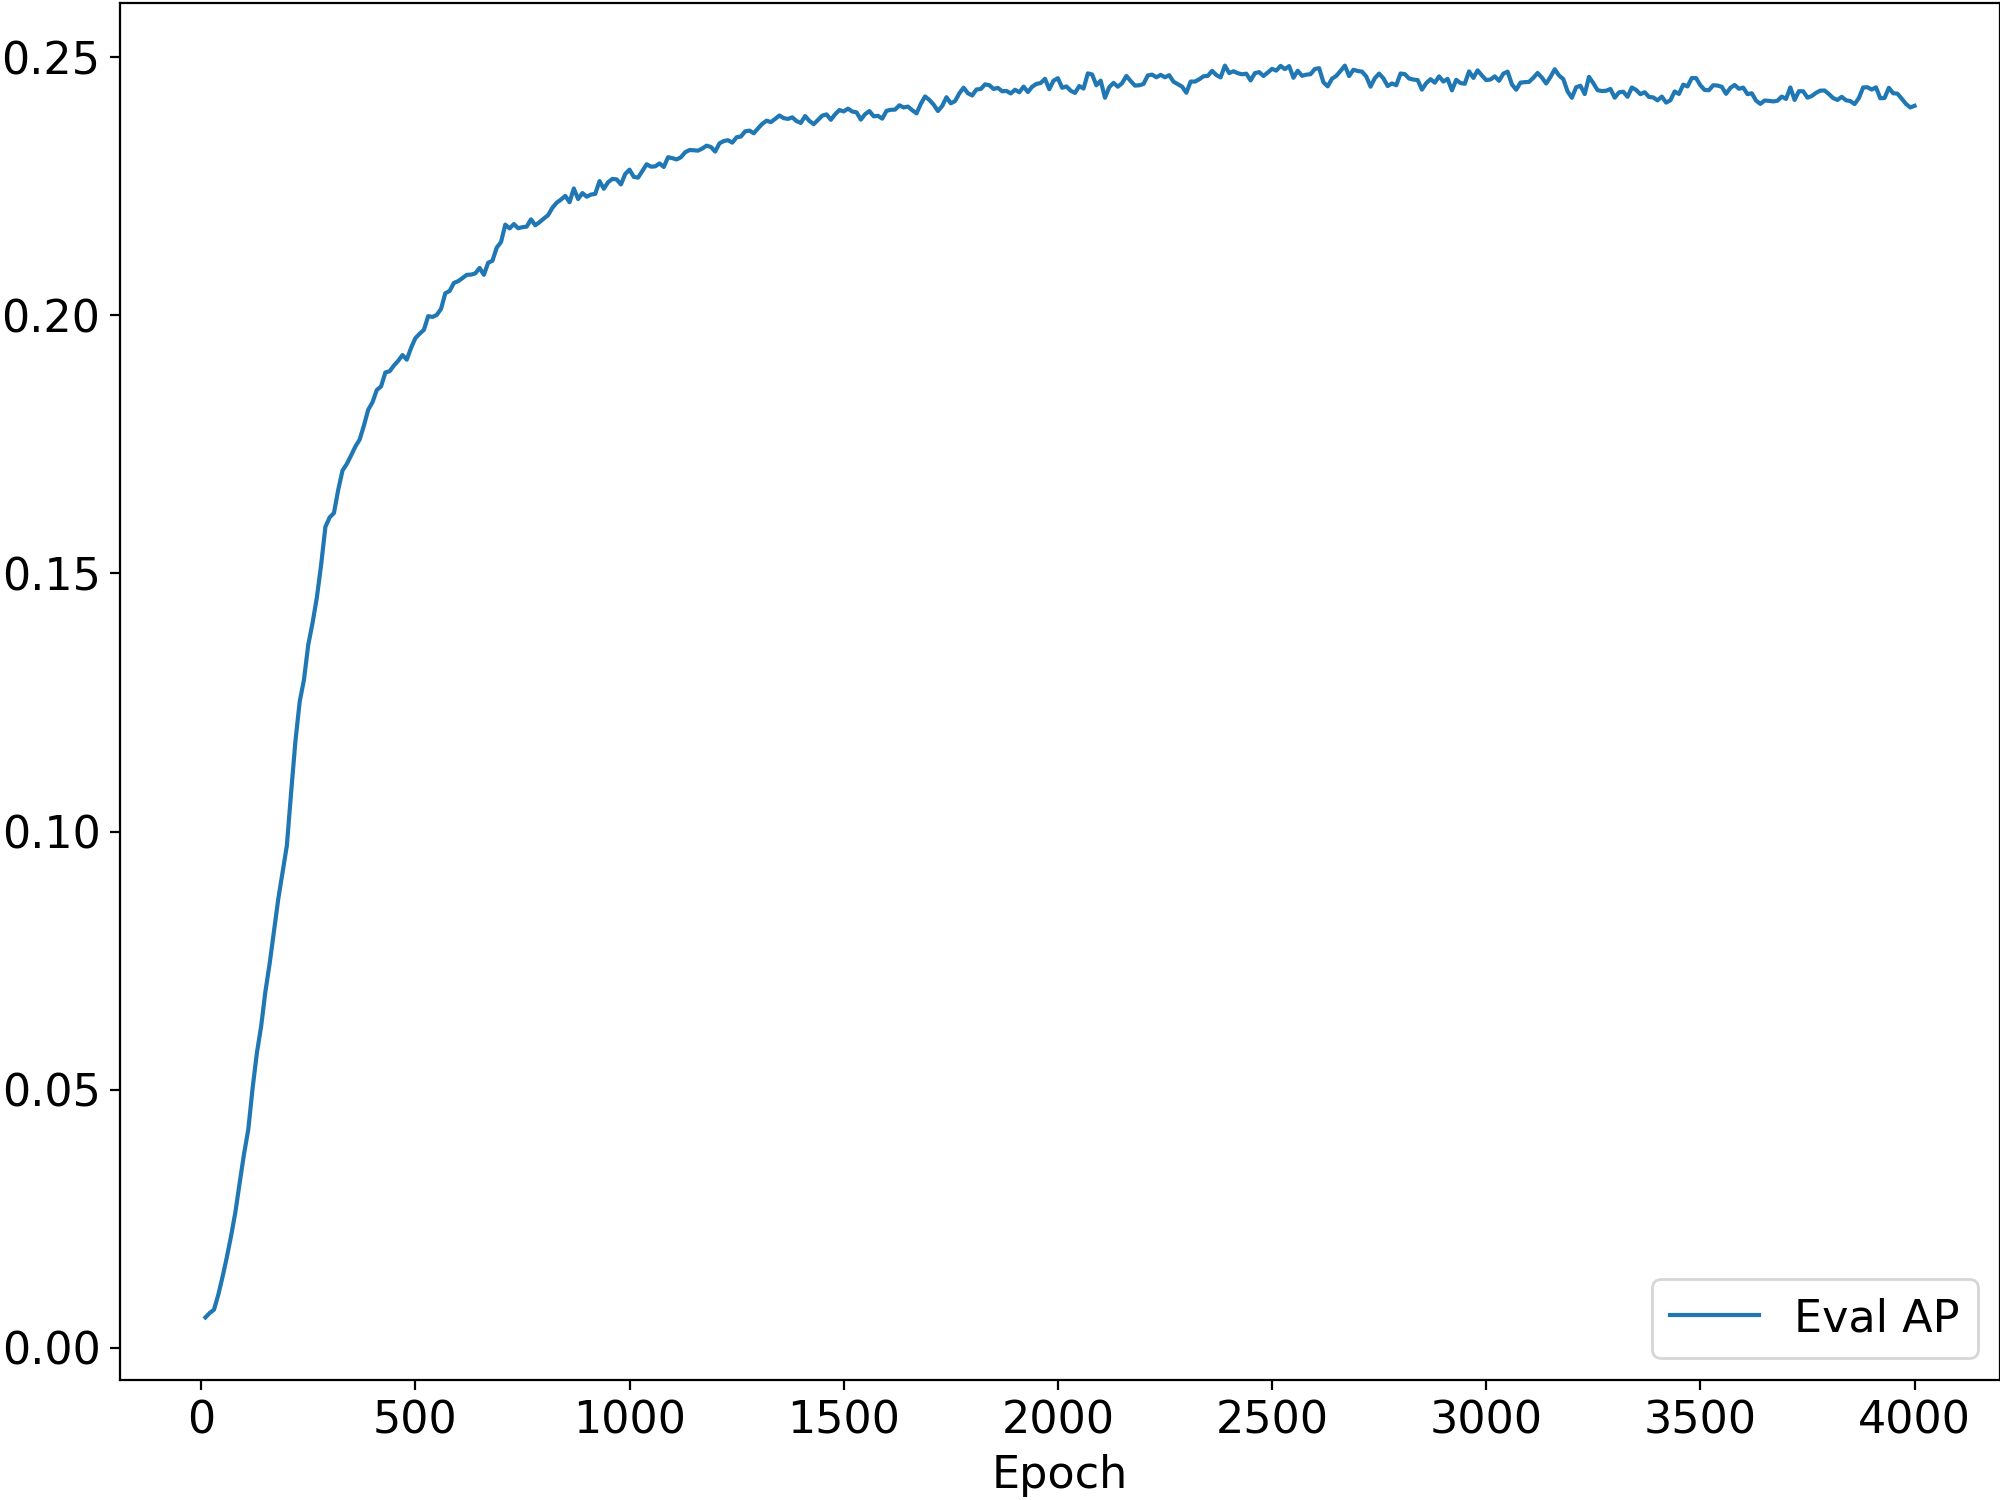
\includegraphics[width=4.8cm]{figures/rnn-AP.png}
					}
					\subfigure[Loss]{
						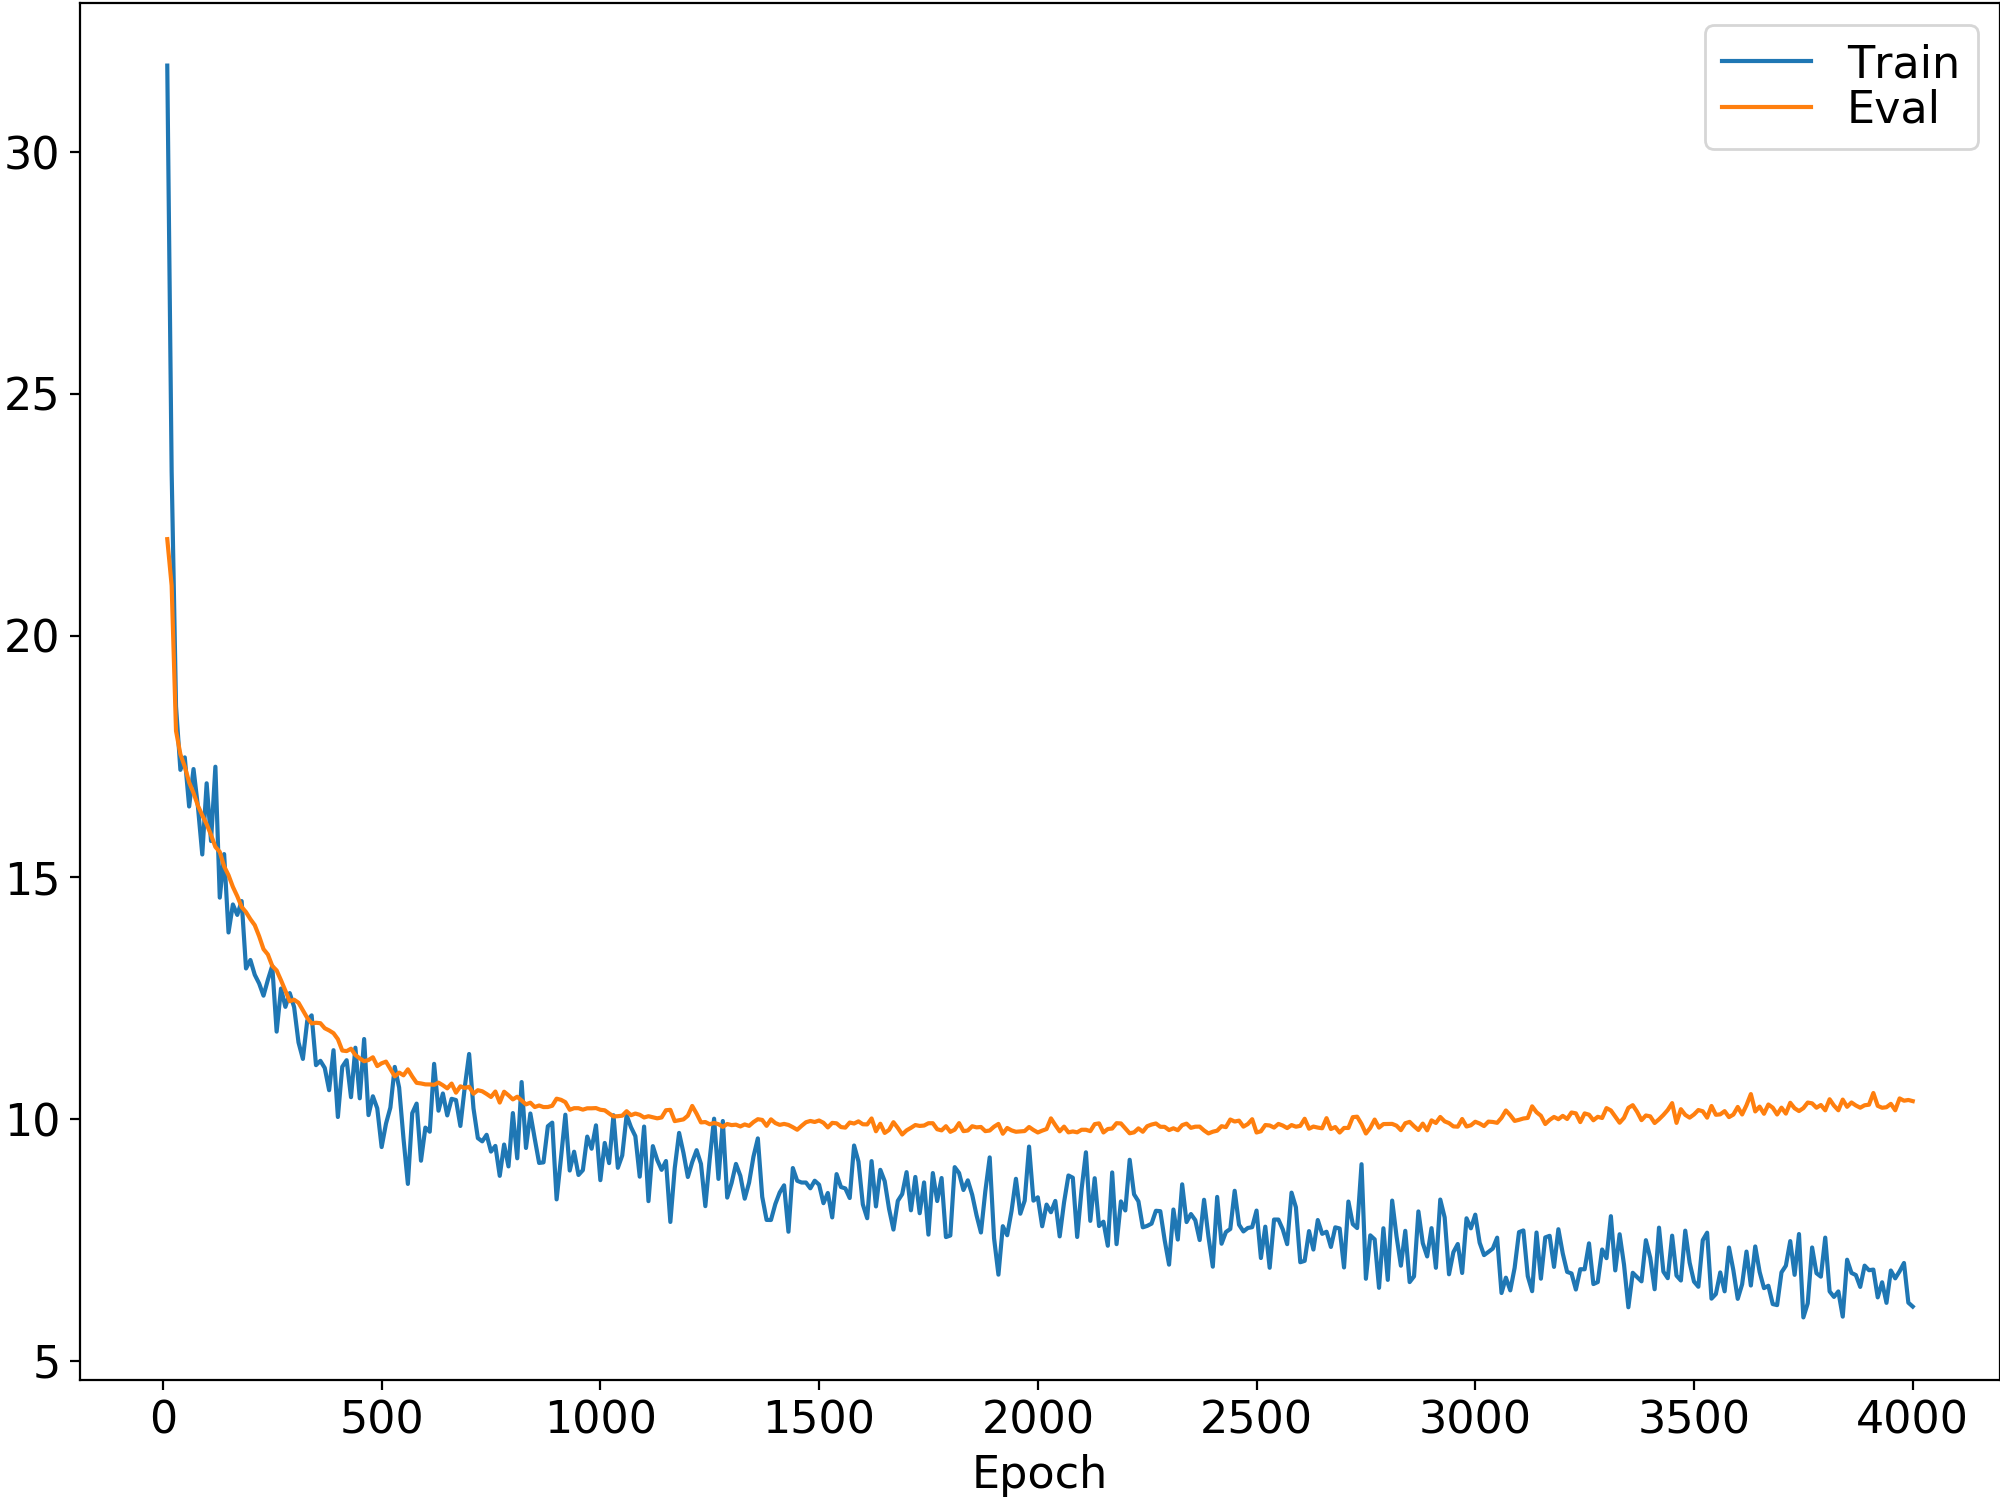
\includegraphics[width=4.8cm]{figures/rnn-loss.png}
					}
					\caption{\label{fig:rnn-proc}Figures on Recurrent Networks}
				\end{figure}
		\subsection{Preventing Overfitting}
			The version of this dataset we used is a small subset of the original AudioSet consisting of only about 20 thousands entries, which means that overfitting problem can be really serious. As the training procedure goes through, the loss on training set is decreased much more quickly than the counterpart on evalution set. We provide the following two idea to prevent overfitting.
			\subsubsection*{Adding Noise to Training Data}
				Adding noise to the training data can slightly extenuate the problem. In our experiments, we made 5 copies of the training data with different Gaussian noise. However, despite this method can only increase the robustness of the training process, the performance does not benefit from it. One hypothesis is that neural networks can easily learn to know that the data is noisy and can automatically calculate the deviation and the mean value of the noise. Proving this hypothesis is remained as future works.
			\subsubsection*{Double Training Data by Time Inversion}
				This idea is inspired by the similar idea in the computer vision field that the problem of lacking data can be eased by flipping and adjusting light. However, though audio is sequential, this method does not bring any improvement on the final performance.
		\subsection{Platform Speed Comparation}
			\subsubsection*{Environment Settings}
				We compared the speed of DNN using three mainstream deep learning programming frameworks on a machine with 16 CPU and one GeForce GTX 1080 Ti GPU card.
			\subsubsection*{Results}
				The table \ref{table:performance} shows elapsed CPU time and performances of the three frameworks.
				\begin{table}[htbp]
					\centering
					\begin{tabular}{c|ccc}
						\hline
						\hline
						 Batch Size      & Tensorflow & MXNet & PyTorch\\
						\hline
						    Performance  &   94.5/0.242 & 94.4/0.242 & 93.3/0.206 \\
						    Elapsed Time(s) & 45.85  & 37.78  & 26.46 \\
						\hline
					\end{tabular}
					\caption{\label{table:performance}Experiments on Comparing Frameworks' Performance}
				\end{table}
		\subsection{Ensemble Experiments}
			We use the ensemble methods of averaging weights among all of the good models (having AUC larger than 94). Finally we get the best model with AUC $94.9$ and AP $0.257$ compared to the best model with AUC $94.4$ and AP $0.241$ listed in table \ref{table:ensemble}.
			\begin{table}[htbp]
					\centering
					\begin{tabular}{l|cc}
						\hline
						\hline
						 Model Type  & AUC & AP\\
						\hline
						  3-Conv-Layers CNN           &  94.2 & 0.236 \\
						  10-Layers 2048-Units RNN    &  94.3 & 0.247 \\
						  Single Layer DNN            &  94.4 & 0.241 \\
						\hline
						  Total                       &  94.9 & 0.257 \\
						\hline
					\end{tabular}
					\caption{\label{table:ensemble}Ensemble Models}
				\end{table}
	\section{Discussion and Future works}\label{sec:discuss}
		In this paper, we compared three basic neural network architectures, DNN, CNN and RNN on Google AudioSet, among which single layer DNN performs the best. However, with fine tunning the parameters, RNN and CNN are not worse than the single-layer DNN. 

		Besides, ensemble methods can truly improve the performance and this performance is better than the best performance among all models. However, due to the networks learning homogeneously, the averaging ensemble method did not bring a remarkable improvement on the final performance.

		In the experiments of platform comparison, PyTorch is the fastest framework. But here we only tested single layer neural network while Tensorflow performs the best. Comparing more sophiscated networks is remained as future works.

		Future works includes trying other complicated neural networks such like the combination layer of convolutional layer and recurrent layer as well as the other multi-label problem transformations such as learn the pairwise probability that label $i$ is more likely to be selected compaired with lable $j$. Besides, having exploration on other datasets and trying the other ensemble methods are also worth a try.

	\newpage
	\bibliographystyle{unsrt}
	\bibliography{paper}

\end{document}
